%% -*- mode: latex; mode: reftex; mode: flyspell; coding: utf-8; tex-command: "pdflatex.sh" -*-

%% Any copyright is dedicated to the Public Domain.
%% https://creativecommons.org/publicdomain/zero/1.0/
%% Written by Francois Fleuret <francois@fleuret.org>

\documentclass[11pt,a4paper,oneside]{article}
\usepackage[paperheight=15cm,paperwidth=8cm,top=2mm,bottom=15mm,right=2mm,left=2mm]{geometry}
% \usepackage[a4paper,top=2.5cm,bottom=2cm,left=2.5cm,right=2.5cm]{geometry}
\usepackage[utf8]{inputenc}
\usepackage{amsmath,amssymb,dsfont}
\usepackage[pdftex]{graphicx}
\usepackage[colorlinks=true,linkcolor=blue,urlcolor=blue,citecolor=blue]{hyperref}
\urlstyle{same}
\usepackage{tikz}
\usetikzlibrary{arrows,arrows.meta,calc}
\usetikzlibrary{patterns,backgrounds}
\usetikzlibrary{positioning,fit}
\usetikzlibrary{shapes.geometric,shapes.multipart}
\usetikzlibrary{patterns.meta,decorations.pathreplacing,calligraphy}
\usetikzlibrary{tikzmark}
\usetikzlibrary{decorations.pathmorphing}
\usepackage[round]{natbib}
\usepackage[osf]{libertine}
\usepackage{microtype}

\usepackage{mleftright}

\usepackage{enumitem}
\setlist[itemize]{leftmargin=0pt,itemindent=1em,itemsep=2ex}
\setlist{nosep} % or \setlist{noitemsep} to leave space around whole list

\newcommand{\setmuskip}[2]{#1=#2\relax}
\setmuskip{\thinmuskip}{1.5mu} % by default it is equal to 3 mu
\setmuskip{\medmuskip}{2mu} % by default it is equal to 4 mu
\setmuskip{\thickmuskip}{3.5mu} % by default it is equal to 5 mu

\setlength{\parindent}{0cm}
\setlength{\parskip}{1ex}
%\renewcommand{\baselinestretch}{1.3}
%\setlength{\tabcolsep}{0pt}
%\renewcommand{\arraystretch}{1.0}

\def\argmax{\operatornamewithlimits{argmax}}
\def\argmin{\operatornamewithlimits{argmin}}

%%%%%%%%%%%%%%%%%%%%%%%%%%%%%%%%%%%%%%%%%%%%%%%%%%%%%%%%%%%%%%%%%%%%%%

\def\given{\,\middle\vert\,}
\def\proba{\operatorname{P}}
\newcommand{\seq}{{S}}
\newcommand{\expect}{\mathds{E}}
\newcommand{\variance}{\mathds{V}}
\newcommand{\empexpect}{\hat{\mathds{E}}}
\newcommand{\mutinf}{\mathds{I}}
\newcommand{\empmutinf}{\hat{\mathds{I}}}
\newcommand{\entropy}{\mathds{H}}
\newcommand{\empentropy}{\hat{\mathds{H}}}
\newcommand{\ganG}{\mathbf{G}}
\newcommand{\ganD}{\mathbf{D}}
\newcommand{\ganF}{\mathbf{F}}

\newcommand{\dkl}{\mathds{D}_{\mathsf{KL}}}
\newcommand{\djs}{\mathds{D}_{\mathsf{JS}}}

\newcommand*{\vertbar}{\rule[-1ex]{0.5pt}{2.5ex}}
\newcommand*{\horzbar}{\rule[.5ex]{2.5ex}{0.5pt}}

\def\positionalencoding{\operatorname{pos-enc}}
\def\concat{\operatorname{concat}}
\def\crossentropy{\LL_{\operatorname{ce}}}

\begin{document}

\vspace*{-3ex}

\begin{center}
{\Large Self-Generated Culture}

Fran\c cois Fleuret

\today

\vspace*{2ex}

\centerline{\color{red}(work in progress, to be updated)}

\medskip

\centerline{\url{https://fleuret.org/public/culture/culture.pdf}}

\end{center}

\section{Introduction}

The hypothesis behind this experiment is that high-level abstract
thinking is fueled by social competition. A group of communicating
agents that try to demonstrate their cognitive superiority would end
up developing a rich and consistent culture.

The experiment is designed with a group of GPTs that alternatively
learn to solve quizzes and generate new ones.

A ``quiz'' is a triplet of the form $(A, d, B)$ where $A$ and $B$ are
two sequences and $d$ is a token indicating if the direction is
forward or backward. Given $(A, d)$, the challenge is to generate $B$.

The experiments starts with a set of quizzes, that is going to be
progressively enriched.

\section{Bird World}

The initial set of quizzes consist of predicting the dynamics of a
very simple world: A $6 \times 8$ grid with three colored ``birds'' moving in
a straight line, possibly bouncing on the grid's borders. There are
ten different colors.
%
\begin{center}
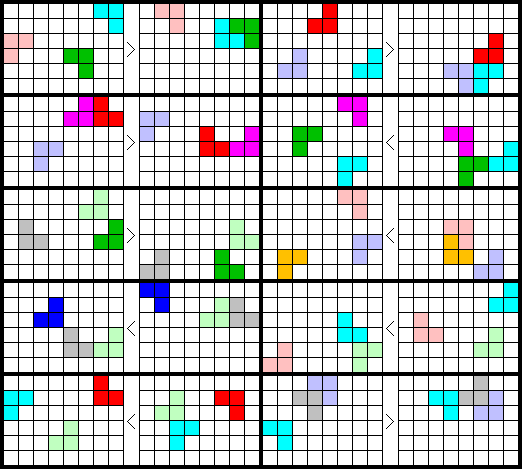
\includegraphics[scale=0.35]{pics/examples_train.png}
\end{center}
%

\vspace*{-2ex}

In each on these quizzes, $A$ is the left image serialized in
raster-scan order as a sequence of $6 \times 8 = 48$ tokens, $d$ is
either the token ``forward'' or the token ``backward'', and $B$ is the
right image, also serialized. The direction of prediction is chosen at
random.

\section{Generating Quizzes}

Given a set of $N$ GPTs, we can generate new quizzes as follows:
Select one of the models, and use it to generate the $97$ tokens of a
triplet $(A, d, B)$.

Then with each one of the $N-1$ other models, predict $B$ from $(A,
d)$, and $A$ from $(B, d')$ where $d'$ is the direction token opposite
of $d$.

A quiz is validated if \textbf{all the other GPTs but one predict it
  deterministically correctly in both directions.}

This criterion assures that the new quizzes are both solvable and
sophisticated, and incrementally complexify the culture. Imposing both
direction prevents the generation of quizzes which are not trivial
only because the prompt has been randomly degraded.

\section{Overall Process}

The overall process consists of training the GPTs from scratch by
iterating the following steps:
%
\begin{itemize}

\item select the GPT with the lowest recorded test accuracy, train it through one epoch,

\item if its test accuracy gets above $97.5\%$, generate $1'000$ new
  quizzes, add them to the training set, re-compute the accuracy of
  all the models

\end{itemize}

\section{Results}

This procedure results in the discovery of patterns which are not
present in the original quizzes:

\textbf{More birds}

\begin{center}
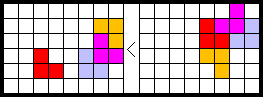
\includegraphics[scale=0.35]{pics/4_birds_1.png}
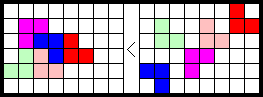
\includegraphics[scale=0.35]{pics/5_birds_1.png}

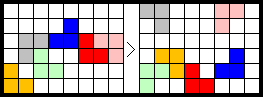
\includegraphics[scale=0.35]{pics/6_birds_1.png}
\end{center}

\textbf{New bird shapes}

\begin{center}

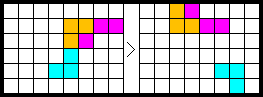
\includegraphics[scale=0.35]{pics/other_shapes_2.png}
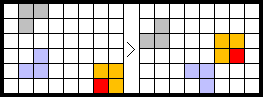
\includegraphics[scale=0.35]{pics/other_shapes_3.png}
\end{center}

\textbf{Occlusions}

\begin{center}
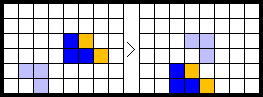
\includegraphics[scale=0.35]{pics/other_shapes_1.png}
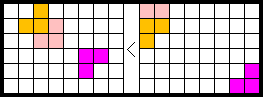
\includegraphics[scale=0.35]{pics/occlusions_1.png}
\end{center}

\section{Various thoughts}

\begin{itemize}

\item The whole process can be envisioned as natural selection of
  quizzes in the representation landscape of GPTs. There probably is a
  subtle relation between the temperature (mutation rate) and the
  number of models used to validate with the ``all but one'' criterion
  (survival criterion).

\item The ``all but one'' could be ``all but K'', and there may be
  some information-theoretical thing, where the goal is to maximize
  mutual information, with $K=N$ being total randomness, so high
  entropy but no structure, and $K=0$ is total determinism, so no
  information to share.

\item The setup does not push toward any specific invariance or
  property in the generated quizzes, their consistency is entirely due
  to the statistics of the ``world quizzes'' that remain in the
  training set, and to the GPTs' inductive biased.

\item The GPTs obviously get a sense of objectness and 2d topology
  early on, since they rapidly increase the number of birds and
  ``discover'' occlusion even though they never was in the world
  quizzes.

\item There may not be so many problems that can be cast as pairs of
  patterns that are each a deterministic function of the other, which
  is probably critical here.

\item This overall process probably fight the ``simplicity bias'': If
  a model is lacking a ``cue'' that the others have, there will
  rapidly be quizzes that require this cue, they will be added to the
  training data, and that model will catch up.

\item The randomness of the process probably allow to even go beyond
  just synchronizing the abilities of the models. There may be some
  additional complexification of quizzes that get accepted by chance.

\item It can be parallelized by dispatching the GPTs across multiples
  nodes, and avoiding a quadratic cost by limiting the validation of
  the quizzes to a subset of them.

\item The current process to generate new quizzes, which simply
  samples them at random is very rudimentary and probably not
  sufficient in a real-data setup. It can probably be supplemented
  with a MCTS-type search.

\item There may be already in the generated quizzes some structure
  that \emph{we} do not pick up (e.g. certain color or motion
  patterns).

\end{itemize}

\section*{Appendix}

The code is available at

\medskip

\centerline{\url{https://fleuret.org/git/culture}}

The experiments are done with a GTX 4090.

The GPT used has 37M parameters and the following structure:

\begin{center}
\begin{tabular}{lc}
    \texttt{dim\_model}  & 512  \\
    \texttt{dim\_keys}   & 64   \\
    \texttt{dim\_hidden} & 2048 \\
    \texttt{nb\_heads}   & 8    \\
    \texttt{nb\_blocks}  & 12
\end{tabular}
\end{center}

Adam, $\eta = 1e-4$, no scheduling.

There are $N_{\text{train}}=250'000$ original quizzes for training and
$N_{\text{test}} = 10'000$ for test.

At each epoch, for both train and test samples, we mix original
quizzes and the generated ones.

For training for instance, if there are less than $N_{\text{train}}/2$
new quizzes, we take all of them, otherwise we sample
$N_{\text{train}}/2$ of them without replacement, and then we sample
without replacement enough original quizzes to get $N_{\text{train}}$
samples in total.

We proceed similarly to get $N_{\text{test}}$ samples for test.

\end{document}
